\documentclass[12pt]{iopart}
\pdfminorversion=4
\newcommand{\gguide}{{\it Preparing graphics for IOP Publishing journals}}
%Uncomment next line if AMS fonts required
%\usepackage{iopams}  
\usepackage{harvard}
\usepackage{graphicx}
\newcommand{\mathbb}[1]{\mathrm{#1}}
\usepackage{xcolor}
\begin{document}

\title[]{Full waveform ultrasound tomography for in-vivo sound speed and reflection imaging}

\author{I E Ulrich$^1$,  C Boehm$^1$,
P Marty$^1$, S Noe$^1$, N Korta Martiartu$^{2,3}$, X L Dean-Ben$^{4, 5}$, D Razansky$^{4, 5}$ and A Fichtner$^1$}

\address{$^1$ Institute of Geophysics, ETH Zurich, Sonneggstrasse 5, 8092 Zurich, Switzerland}
\address{$^2$ Institute of Applied Physics, University of Bern, Sidlerstrasse 5, 3012 Bern, Switzerland}
\address{$^3$ Institut Langevin, ESPCI Paris, PSL University, CNRS, 1 rue Jussieu, F-75005, Paris, France}
\address{$^4$ Institute of Pharmacology and Toxicology and Institute for Biomedical Engineering, University of Zurich, Winterthurerstrasse 190, 8057 Zurich, Switzerland}
\address{$^5$ Institute for Biomedical Engineering, ETH Zurich, Wolfgang-Pauli-Strasse 27, 8049 Zurich, Switzerland}
\ead{ines.ulrich@eaps.ethz.ch}

\vspace{10pt}

\begin{abstract}
	Full-waveform inversion (FWI) is a powerful reconstruction technique for generating high-resolution models of tissue and bone structure using non-invasive ultrasonic measurements. Quantitative information on the model parameters, such as the sound speed in soft tissue, are obtained via an iterative data fitting procedure that accounts for the nonlinear relationship between the ultrasonic wavefield and the model parameters. However, owing to its computational complexity, FWI has yet to see widespread adoption in medical practice. This study applies acoustic FWI to in-vivo data with the objective to showcase the potential gain in resolution of reconstructed models. We identify three key components that are essential to reconstruct such high-resolution models and to accurately identify anatomical features: (1) an accurate model of the source wavelet, obtained by inverting for the source-time function using the calibration data in water; (2) a misfit functional that reduces nonlinearity and dependence on the initial model, which is achieved with a definition of the misfit in terms of graph-space optimal transport; and (3) a resolution analysis based on point perturbations, providing proxies for local spatial smearing of reconstructed features. 
\end{abstract}

%
\vspace{2pc}
\noindent{\it Keywords}: Full-waveform inversion, image reconstruction, in-vivo data, reflection imaging, resolution analysis, sound speed estimation, ultrasound tomography.
%
% Uncomment for Submitted to journal title message
%\submitto{\JPA}
%
% Uncomment if a separate title page is required
%\maketitle
% 
% For two-column output uncomment the next line and choose [10pt] rather than [12pt] in the \documentclass declaration
%\ioptwocol
%


\section{Introduction}
\label{sec:introduction}
Medical ultrasound offers the possibility to generate qualitative images of impedance contrast in tissue delineating internal structure, as well as quantitative images of the tissue parameters. The low operational costs, combined with the non-ionizing nature of ultrasonic waves and the ability to design portable devices, enable a wide range of applications. This is particularly true for high-throughput, recurring scanning procedures for instance in the context of tumor growth monitoring.

To learn about the internal properties of tissue using recorded ultrasonic waves, one may take two approaches: (1) focus on particular phases in the measured data, specifically the first arrivals in transmission or reflection, or (2) consider the entire wavefield. Approach one is the subject of conventional pulse-echo, or reflection ultrasound methods, where the travel time is computed using a linearized wave propagation model assuming single scattering. A prominent example is the delay-and-sum algorithm \cite{Jensen_2006,Gemmeke_2017}, which produces images of impedance contrasts within the tissue. Information on tissue parameters such as sound speed or attenuation may be obtained with ray tomography \cite{Gemmeke_2017} that exploits the first arrivals of transmitted waves. In contrast to this, waveform-based imaging approaches aim to exploit the full time series of an ultrasound measurement to extract information on tissue parameters, hence the name full-waveform inversion (FWI). This holistic consideration of the wavefield is motivated by the fact that first arrivals constitute only a fraction of the measured signals with a large majority of data being contained in reflected, diffracted, and scattered waveforms encoding information on the tissue structure off the direct ray path. 

In FWI, a model of the tissue properties is constructed via an iterative inversion process that harnesses numerical solutions to the wave equation to minimize their misfit with respect to the observed data \cite{Tarantola_1984_2,Virieux_Operto_2009,Fichter_FWI_book_2011}. Taking into account sparse coverage, noise, attenuation, and realistic transducers, FWI can achieve a spatial resolution close to the diffraction limit, thus on the order of half the shortest wavelength \cite{Devaney_1984}. This is higher than for ray tomographic methods where the spatial resolution is limited by the source receiver distance and frequency content of the experiment defining the width of the first Fresnel zone \cite{Schatzberg_Devaney_1992,Cerveny_2001}. The ability of FWI to reconstruct tissue properties such as sound speed or attenuation accurately from medical ultrasound data has been demonstrated for laboratory measurements \cite{KortaMartiartu_2020}, photoacoustic imaging \cite{Huang_2013,Mitsuhasi_2017}, soft tissue imaging \cite{Pratt_Duric_2007,Wiskin_2020} as well as transcranial ultrasound \cite{Guasch_2020,Marty_SPIE_2021,Mitcham_2023}. 

The adoption of FWI methods for real data, however, has so far been impeded by the narrow bandwidth of common ultrasound transducers and the need for accurate starting models. Both of these aspects are related to the non-convex nature of the misfit characterized by local minima, which are difficult to handle in gradient-based optimization procedures typically employed in FWI. Additionally, a central aspect of accurately simulating the ultrasonic wavefield is precise knowledge of the source-time function, yet manufacturer-provided source-time functions are often insufficient in accuracy for use in FWI. Lastly, a resolution analysis in FWI is challenging since the data depend nonlinearly on the model. The latter implies that strategies used to describe the posterior in linear inverse problems are not applicable to FWI. The objective of this study is therefore threefold: (1) to broaden the range of applicability of FWI for real devices by defining a more robust measure of misfit that can mitigate cycle skipping and allows for less informative starting models; (2) to increase the tomographic resolution by performing an auxiliary inversion for the source-time function; and (3) to propose a strategy for a resolution analysis that is applicable in practice without significantly adding to the computational costs.    

We demonstrate the effectiveness of the proposed concepts with a time-domain acoustic full-waveform inversion using an in-vivo ultrasound data set of a mouse. The acquisition device is a transmission-reflection optoacoustic ultrasound imaging platform \cite{lafci_IEEE_TUFFC}, which allows for the joint imaging of optical absorption, ultrasound reflectivity, and acoustic properties of the tissue. To overcome the tendency of FWI to stall in a local minimum, we define the misfit in terms of graph-space optimal transport (GOT) \cite{Metevier_GOT_2019}, which can be tuned to alleviate the appearance of local minima. 

To calibrate the source wavelet, we draw inspiration from seismic imaging \cite{Groos_2014} and invert for each source-time function individually in an auxiliary linear inversion. This takes advantage of the water shot, which is routinely collected during data acquisition. With this setup, the tissue sound speed map can be reconstructed with high accuracy, allowing for the differentiation between small-scale internal structures delineated in the corresponding reflection image.   

Lastly, we propose a practical method for resolution analysis in order to quantify the quality of the reconstructed images. Our strategy thereby involves inferring curvature information contained in the Hessian of the misfit. With this, point-spread functions can be approximated that assess the local resolution lengths of reconstructed features. To render the proposed resolution analysis applicable in practice, we employ source encoding \cite{Capdeville_2005,Krebs_2009,Wang_2015}, a well-established technique to reduce the computational costs for gradient computations in FWI. 

%=======================================================================================
%%%%%%%%%% THEORY %%%%%%%%%%
%=======================================================================================
\section{Theory}
\label{sec:theory}
%-----------------------------------------------------------------------------------
% Forward Problem
%-----------------------------------------------------------------------------------
\subsection{Forward problem}
The backbone of FWI is the accurate numerical modeling of the propagation of the ultrasonic wavefield. The aim is to estimate a model of the tissue properties $\mathbf{m}$, such as for instance the sound speed $c(\mathbf{x})$ and mass density $\rho(\mathbf{x})$, that predicts a set of measurements of the acoustic pressure $p(\mathbf{x},t)$. We consider a setup where the domain of interest $\Omega$ consists of a water bath with the immersed mouse model enclosed by a transducer array, which delineates the boundary of the domain. For soft tissues, the governing equation for acoustic wave propagation is given by 
\begin{equation}
 \frac{1}{\rho(\mathbf{x}) c^2(\mathbf{x})}\partial_t^2p(\mathbf{x},t)-\nabla\cdot\bigg(\frac{1}{\rho(\mathbf{x})}\nabla p(\mathbf{x},t)\bigg)=\frac{1}{\rho(\mathbf{x})}f(\mathbf{x},t),
 \label{eq:wave_equation_time_domain}
\end{equation}
where $f(\mathbf{x},t)$ denotes the external sources. Neumann, Dirichlet or absorbing boundary conditions may be enforced along different parts of the domain boundary. To discretize \eref{eq:wave_equation_time_domain} we use the spectral-element method \cite{Salvus} and define $\mathbf{p}=[p(\mathbf{x},t)\;\mbox{for}\;t\in[t_0,t_1]\;\mbox{and}\;\mathbf{x} \in \Omega]$ as the pressure wavefield, $\mathbf{L}$ as the discrete wave operator in 2 dimensions and let $\mathbf{f}$ represent a point source scaled by the inverse of the density at that point, which makes it the discrete counterpart to the scalar source-time function on the right-hand side of \eref{eq:wave_equation_time_domain}. In a discrete setting, the pressure wavefield is observed at receiver positions $\mathbf{x}_r$, where $r=1,2,...,n_r$, and is extracted from the total field by application of a restriction operator $\mathcal{R}$, such that $\mathbf{d}=(\mathcal{R}\mathbf{p})_r=p(\mathbf{x}_r,t)$ denotes the simulated wavforms recorded at the receivers. We then write \eref{eq:wave_equation_time_domain} compactly in terms of a matrix vector product 
\begin{equation}
	\mathbf{L}(\mathbf{m};\mathbf{x},t)\mathbf{p}(\mathbf{m})=\mathbf{f}, \quad
	\mathbf{x}\in\Omega\subset\mathbb{R}^N, \;\;t\in[t_0,t_1]\subset\mathbb{R}.
	\label{eq:forward_wave_equation_compact}
\end{equation}
Here, $\mathbf{L}$ is linear in the pressure wavefield $\mathbf{p}$ for a fixed set of model parameters $\mathbf{m}=[\rho(\mathbf{x});c(\mathbf{x})]$ and a given source $\mathbf{f}$. However, the parameter-to-solution map $\mathbf{m}\mapsto\mathbf{p}(\mathbf{m})$ linking the wavefield $\mathbf{p}(\mathbf{m})$ to model parameters $\mathbf{m}$ is nonlinear. 
 
%-----------------------------------------------------------------------------------
% Waveform Inversion
%-----------------------------------------------------------------------------------
\subsection{Full-waveform inversion}
\label{subsec:FWIproblem}
Inverting for $\mathbf{m}$ by modeling the nonlinear relationship of the wavefield with respect to the model parametersis the challenging primary goal of FWI. To this end, FWI is formulated as a nonlinear, local constrained optimization procedure with the objective to minimize the waveform misfit $\chi$ between simulated data $\mathbf{d}(\mathbf{m})=(\mathcal{R}\mathbf{p}(\mathbf{m}))_r$ and the measured data $\mathbf{d}^{\mbox{\scriptsize obs}}$. To efficiently compute directional derivatives of $\chi$ with respect to the model parameters, FWI uses the adjoint method \cite{Tarantola_1988,Pratt_1999_1,Tromp_adjoints_2005}. To construct an augmented objective function $\psi$, a Lagrange multiplier $\mathbf{q}$ can be used to include the constraint, which is the forward equation in \eref{eq:forward_wave_equation_compact}:
\begin{equation}
	\psi(\mathbf{m},\mathbf{p},\mathbf{q})=\chi\big((\mathcal{R}\mathbf{p})_r;\mathbf{d}^{\mbox{\scriptsize obs}}\big)-\mathbf{q}^T\big(\mathbf{L}\mathbf{p}-\mathbf{f}\big).
	\label{eq:Lagrangian_objective}
\end{equation}
\Eref{eq:Lagrangian_objective} is minimized by forcing all partial derivatives to zero. This provides formulations for the gradient in a perturbation direction $\delta\mathbf{m}$, 
\begin{equation}
	\nabla_{\mathbf{m}}\chi(\mathbf{m})\delta\mathbf{m}=-\mathbf{q}^T\nabla_{\mathbf{m}}\mathbf{L}\mathbf{p}\delta\mathbf{m},
	\label{eq:gradient_misfit}
\end{equation}
and the adjoint equation
\begin{equation}
	\mathbf{L}^T\mathbf{q}=\nabla_{\mathbf{p}}\chi,
	\label{eq:adjoint_equation}
\end{equation}
where $\mathbf{q}$ plays now the role of the adjoint wavefield, $\mathbf{L}^T$ is the adjoint wave operator and $\nabla_{\mathbf{p}}\chi$ is the adjoint source. To compute the gradient in \eref{eq:gradient_misfit}, one therefore needs two wavefield simulations: one to solve the forward equation \eref{eq:forward_wave_equation_compact} for a given $\mathbf{m}$ and one to solve the adjoint equation in \eref{eq:adjoint_equation}, propagating the data misfit backward in time simultaneously from all receivers.  
%-----------------------------------------------------------------------------------
% trust-region LBFGS
%-----------------------------------------------------------------------------------
To find the descent direction $\delta\mathbf{m}$, we use a quasi-Newton optimization technique based on trust-region L-BFGS \cite{Boehm_2018} where the misfit functional $\chi(\mathbf{m})$ is approximated quadratically and optimized in the vicinity of the current model, the trust region. Within the L-BFGS approximation, the action of the inverse of the approximate Hessian on a vector can be calculated, which we will exploit during the resolution analysis in section \ref{subsec:resolution_analysis}. 
  
%-----------------------------------------------------------------------------------
% Optimal transport
%-----------------------------------------------------------------------------------
\subsection{Optimal transport misfit functional} 
The shape of the misfit landscape is largely impacted by the choice of $\chi$. In FWI, $\chi$ is commonly defined as the $L_2$ distance between observed and measured data \cite{Tarantola_1988,Pratt_1998}, which is sensitive to amplitude mismatches and inherently dominated by large-amplitude waveforms, amplifying the effects of large differences between predicted and measured data. In addition, valuable information on time shifted waveforms, especially at lower amplitudes, cannot be accounted for with an $L_2$-misfit functional. This makes the $L_2$-misfit functional more sensitive to the nonlinearities with respect to the model parameters and, in realistic scenarios, leads to a phenomenon referred to as cycle skipping \cite{Virieux_Operto_2009,Warner_Guasch_2016}. Perturbing such a cycle-skipped model in any direction may improve the waveform fit to the measured data even though the fit with respect to the global minimum may be worsened. It would therefore be desirable to penalize time as well as amplitude mismatches in order to mitigate the risk of the inversion stalling in a local minimum. 
%---------- 
\begin{figure}[!h]
  \centering
  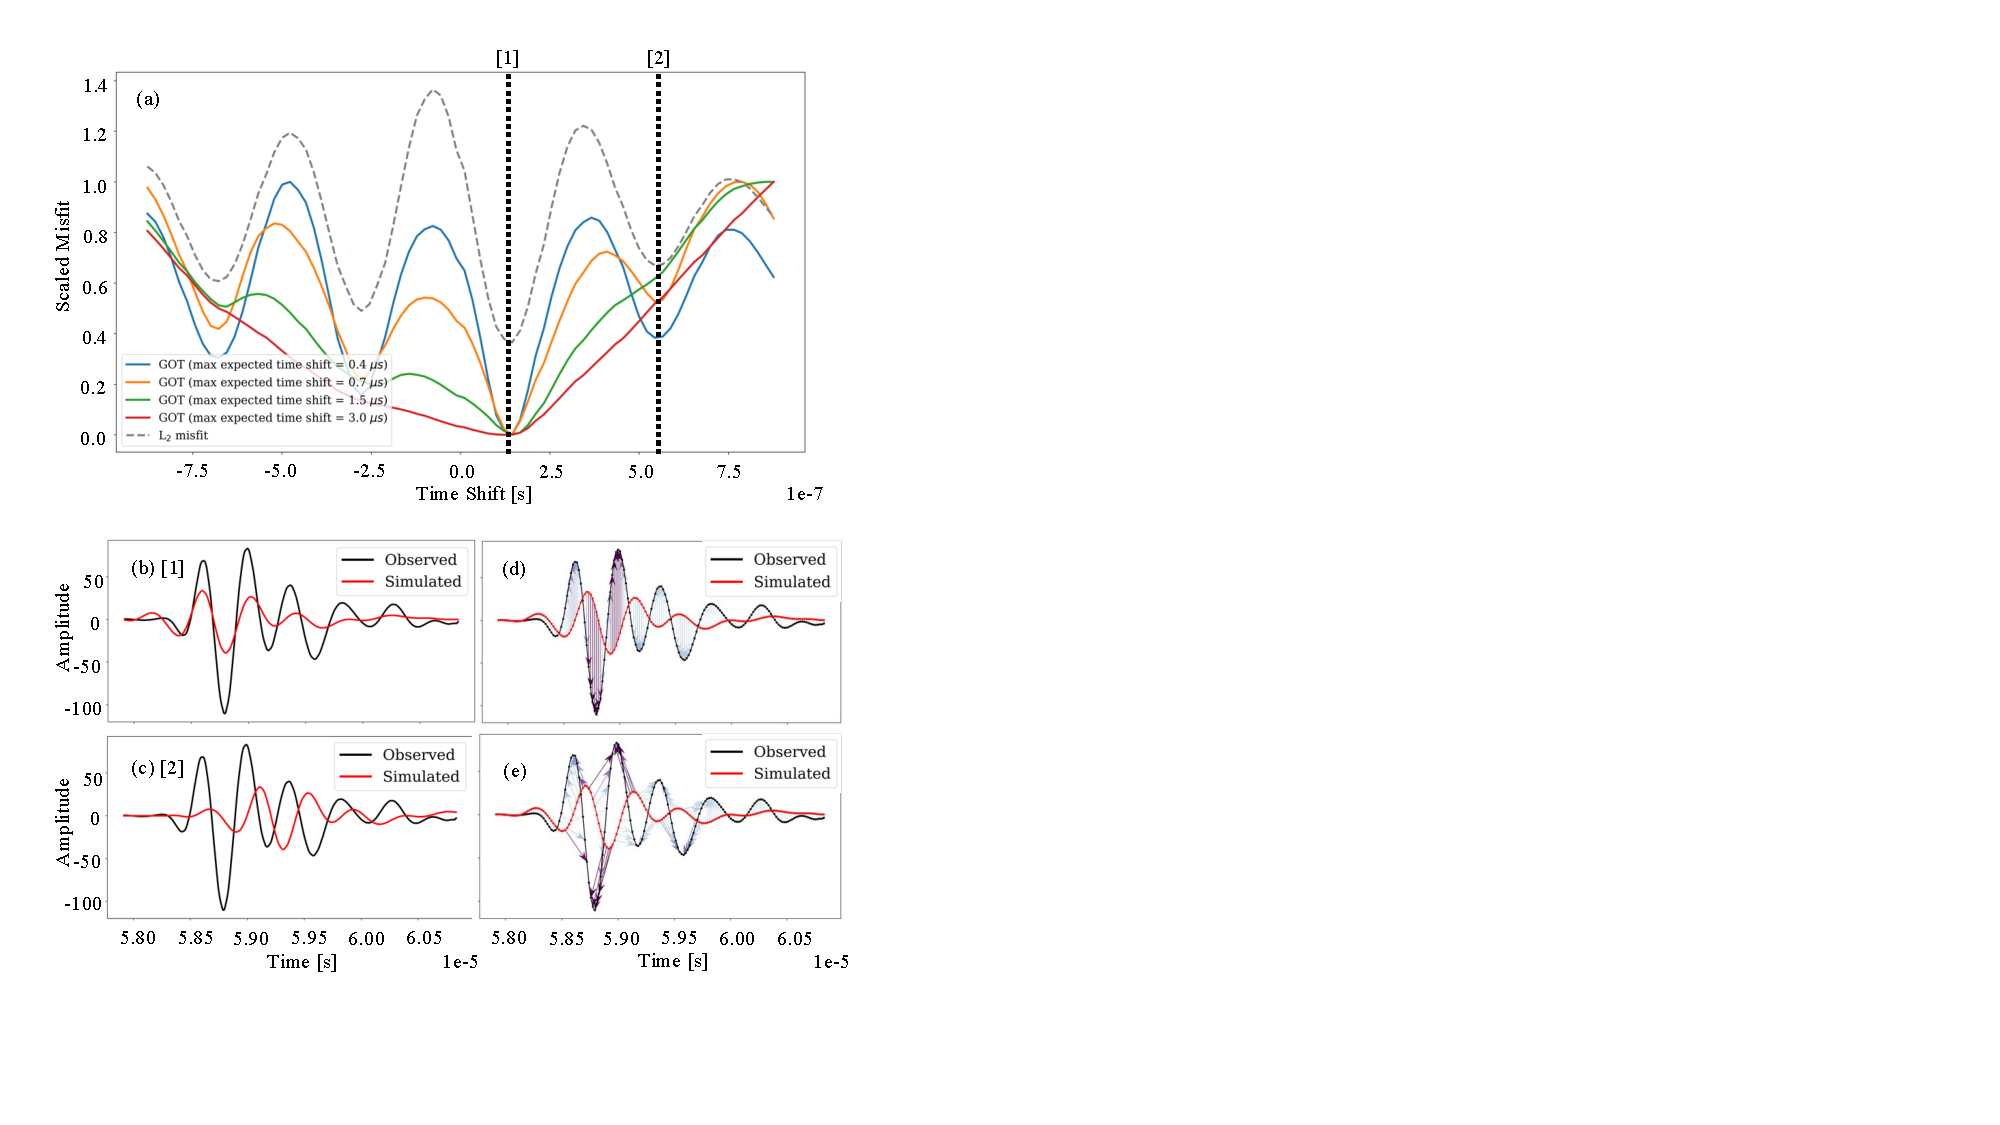
\includegraphics[width=0.9\textwidth]{figure1.pdf}
  \caption{(a) Optimal transport misfit for two time-shifted signals using different values for the tuning parameter (maximum expected time shift). Choosing a larger maximum time shift for the GOT misfit functional eliminates the local minima and widens the valley of attraction. (b) and (c) show one signal of simulated and observed data, shifting the simulated trace to [1] optimally fit the data or [2] to be cycle skipped. (d) and (e) Point cloud matching between a signal of observed and simulated data using different values for the tuning parameter. The color of the arrows indicates the cost of the assignment in graph space. The darker the color, the higher the cost of the assignment. (d) A small tuning parameter associates higher costs to moving points in time, effectively reproducing the behavior of an $L_2$ misfit. The tuning parameter corresponds here to the maximum expected time shift chosen for the blue curve in \fref{fig:MisfitevolutionGOT}(a). (e) Increasing the maximal expected time shift reduces the cost of moving points in time.}
  \label{fig:MisfitevolutionGOT}
\end{figure}
%---------- 
Graph-space optimal transport (GOT) as introduced by Métevier \textit{et al.} \cite{Metevier_GOT_2019} offers such a robust misfit measure, since, instead of comparing waveforms directly, GOT compares the graphs of the waveforms in a 2D graph space. The amplitude-time samples of individual signals are thereby mapped to discrete point clouds, representing the nodes in a graph. The distance between individual points of the two sets has now two components: amplitude and time. The aim of GOT is to find the optimal transport plan that matches points between point clouds pair-wise such that the total cost is minimized. The cost is defined as the cumulative space-time distance across all pairs, where the space component is equal to the amplitude difference and the time component represents the time shift between two samples. An effective measure for the transport cost from one point cloud to another is the Wasserstein metric, which, in contrast to $L_2$, takes into account the geometry of the space where the point clouds are defined. The matching field is then computed by solving an auxiliary optimization problem for the computation of the misfit, reformulated as a Linear Sum Assignment Problem (LSAP) \cite{Boehm_OPT_2022}. The solution to the LSAP defines a permutation of the discrete point cloud for the measured data that contains the information of the point-wise mapping between measured and synthetic signals. Mathematically, this leads to the attractive feature that for two compared signals, the GOT misfit can be adapted to be convex with respect to shifted waveforms. This mapping, however, is not static, but can be tuned by weighting the distance in amplitude versus the distance in time. The resulting tuning parameter defines the convexity of the misfit functional, and thus, provides a robust measure for mitigating cycle skipping. \Fref{fig:MisfitevolutionGOT}(a) shows how different choices of the tuning parameter widen or steepen the valley of attraction, comparing a signal of observed data to time-shifted versions of a simulated signal, taken from the in-vivo FWI inversion results presented in section \ref{subsec:InversionandResults}. The minimum indicates that the simulated signal must be shifted by around 1.5 $\mu$s in order to optimally fit the observed signal as indicated by the line [1] and seen in \fref{fig:MisfitevolutionGOT}(b). Shifting the simulated data by 5.2 $\mu$s results in cycle-skipping as indicated by the line [2] and \fref{fig:MisfitevolutionGOT}(c). \Fref{fig:MisfitevolutionGOT}(d) and (e) display the point cloud matching for two time shifted signals. A small maximum time shift of 0.4 $\mu$s results in high costs on matching points in time and thus increasing the weight on amplitude mismatches, effectively replicating an $L_2$ misfit. Contrarily, increasing the value for the maximum expected time shift allows for permutations that match points in time, which enables time-shifted peaks and troughs to be mapped to their correct counterparts in the observed signal.

Computationally, GOT is more demanding compared to least-squares or cross-correlation misfit functionals. Métivier \textit{et al.} \cite{Metevier_GOT_2019} indicate an increase of 6\% in computational cost of GOT compared to a least-squares misfit functional, based on numerical data. For real data with time-shifted and distorted waveforms, it is therefore attractive to first start the inversion at relatively low frequencies with a GOT misfit functional, using a large maximum expected time shift (assuming the starting model is rather far from the optimal model), and then subsequently decrease the tuning parameter during the inversion. Once sufficient progress has been made in model space, one may switch to a least-squares misfit functional for the final iterations to speed up convergence. We adopt this strategy for our in-vivo FWI in section \ref{subsec:InversionandResults}.

%-----------------------------------------------------------------------------------
% RTM
%-----------------------------------------------------------------------------------
\subsection{Reflection imaging using reverse-time migration}
\label{subsec:RTM}
In medical ultrasound, reflection images are commonly acquired via beamforming techniques using, for instance, delay-and-sum (see \fref{fig:setup_shotgather_traces}(b)). These methods are based on ray theory and thus ignore finite frequency effects, making them efficient to obtain structural images for high-frequency data ($>$1 MHz) \cite{Stotzka_resolution_2005}. In this study, we apply reverse-time migration (RTM) \cite{Levin_RTM_1984,Roy_RTM_2016}, which is a backpropagation technique leveraging numerical solutions to the wave equation. Both, RTM and FWI build on the same imaging condition that correlates the forward wavefield and the adjoint wavefield \cite{Chattopadhyay_McMechan_RTM_2008,Dai_Schuster_2013} to generate an image $I(\mathbf{x})$ of either the reflectivity distribution (RTM) or the model parameter values (FWI). For RTM, the adjoint wavefield is equal to the time-reversed measured wavefield $q(\mathbf{x},T-t)$ propagated from the receivers. The image $I(\mathbf{x})$ is then formed by summing the contribution from all sources 
\begin{equation}
    I(\mathbf{x})=\sum_s\sum_{t=0}^T\partial^2_t p(\mathbf{x},t)q(\mathbf{x},T-t).
    \label{eq:RTM_imaging_condition}
\end{equation}
This allows us to generate a reflectivity image with the same setup that is used for the sound speed inversion by solely changing the definition of the misfit functional $\chi$ in \eref{eq:adjoint_equation}. Douma \textit{et al.} \cite{Douma_2010} show that when the first arrival is removed, the background medium is smooth and when defining $\chi$ to be the least-squares misfit between the forward propagated simulated wavefield and the adjoint wavefield, the image $I(\mathbf{x})$ is given by the impedance kernel.   


%-----------------------------------------------------------------------------------
% Source inversion
%-----------------------------------------------------------------------------------
\subsection{Source-wavelet estimation}
\label{subsec: source_inversion}
A crucial aspect for any real data waveform inversion is an accurate description of the source wavelet used to generate the simulated data \cite{Cueto_sourcecalibration_2020}. To account for individual transducer characteristics, we perform a source inversion prior to each frequency band during the multiscale inversion. We take hereby inspiration from seismic imaging where inverting for the source mechanism is often necessary to account for the complex nature of seismic sources \cite{Pratt_1999_1,Groos_2014}. Formulated as a least-squares problem, the source inversion essentially performs a deconvolution of the instrument response (in its more stable formulation known as a water-level deconvolution \cite{Langston_1979}) from the measured data to isolate the source wavelet for each transducer. We hereby profit from the typically available reference water shot, where the recorded signals are merely a convolution of the source wavelet with the homogeneous Green's function, and the noise spectrum.    

To formulate the auxiliary inverse problem, we let $\hat{\mathbf{d}}_{\mbox{\scriptsize obs}}^k$, $k=1,\ldots,n_r,$ denote the (discrete) Fourier transforms of measured time-domain signals at the $k$-th receiver. Starting from an initial estimate of the source wavelet $\mathbf{f}$, a set of simulations for $k$ receivers are generated and transformed to their frequency domain equivalent $\hat{\mathbf{d}}_{\mbox{\scriptsize sim}}^k$. What we seek is a correction filter $\mathbf{c}$ that, when applied to the initial wavelet, results in a corrected source wavelet $\hat{\mathbf{f}}_{\mbox{\scriptsize opt}} = ({c}_i\,\hat{f}_i)_{i=1}^l$ for each frequency $l$. The simulated data generated by the corrected source $\hat{\mathbf{f}}_{\mbox{\scriptsize opt}}$ has then an improved fit to the measured data $\hat{\mathbf{d}}_{\mbox{\scriptsize obs}}^k$ in a least-squares sense. This in turn implies that the vector of optimized coefficients $\mathbf{c}$ is obtained as the solution of the regularized least-squares problem
\begin{equation}\label{eq:lsq-c}
    \min_{\mathbf{c}} \sum_{k=1}^{n_r} w_k^2 \|  \hat{\mathbf{d}}_{\mbox{\scriptsize obs}}^k - \mathbf{c}\, \hat{\mathbf{d}}_{\mbox{\scriptsize sim}}^k  \|^2 + \alpha \,n_r \| \mathbf{c} \|^2, 
\end{equation}
with $\alpha > 0$ being a regularization parameter. Prior knowledge on individual transducer characteristics, such as the opening angle, the distance between the emitters, as well as prior knowledge on potentially a transducer-dependent signal-to-noise ratio can be adapted by changing the weights $\mathbf{w}= (w_k)$. Let $W$ be the average power of the coefficients $\hat{\mathbf{d}}_{\mbox{\scriptsize sim}}^{k}$ defined as the weighted, normalized $L_2$ norm of the simulated signals
\begin{equation}
    W = \frac{1}{n_r}\sum_{k=1}^{n_r} w_k^2 \| \hat{\mathbf{d}}_{\mbox{\scriptsize sim}}^{k} \|^2.
\end{equation}
We then obtain the coefficients solving \eref{eq:lsq-c} at each discrete frequency $\omega_l$ by using a thresholding parameter $\varepsilon > 0$ and defining $\alpha = \varepsilon^2 W$, resulting in 
\begin{equation}
    c_l = \left(n_r W \varepsilon^2 + \sum_{k=1}^{n_r} w_k^2 | \hat{d}_{\mbox{\scriptsize sim}}^{k,l} |^2 \right)^{-1} \,\left( \sum_{k=1}^{n_r} w_k^2  (\hat{d}_{\mbox{\scriptsize sim}}^{k,l})^* \hat{d}_{\mbox{\scriptsize obs}}^{k,l}  \right).
\end{equation}

%-----------------------------------------------------------------------------------
% Resolution analysis
%-----------------------------------------------------------------------------------
\subsection{Resolution analysis for FWI}
\label{subsec:resolution_analysis}
Ideally, any tomographic image should be complemented by a statement about its resolution. In contrast to linear ray-based techniques, there exists no closed-form solution that allows us to compare prior and posterior information contents for nonlinear waveform inversion \cite{Ulrich_2023}. We can, however, exploit curvature information of the misfit functional to learn more about the characteristics of the minimum. We hereby build on the second-order approximation of the misfit within L-BFGS, where the Hessian $\mathbf{H}$ describes the change of the misfit when the optimal model $\mathbf{\tilde{m}}$ is slightly perturbed to $\mathbf{\tilde{m}}+\delta\mathbf{m}$. 

In the image domain, the information contained in the Hessian therefore encodes inter-parameter blurring and position- and direction-dependent resolution lengths. For realistic-sized problems, the computation of the Hessian matrix is, however, often not possible. Instead, the change in sensitivity of the misfit with respect to a particular perturbation can be analyzed by approximating Hessian-vector products with gradient information in the vicinity of the optimal model    
\begin{equation}
	\mathbf{H}(\mathbf{\tilde{m}})\delta\mathbf{m}\approx\nabla\chi(\mathbf{\tilde{m}}+\delta\mathbf{m})-\nabla\chi(\mathbf{\tilde{m}}),
	\label{eq:Hesse-vector_product}
\end{equation}
where the gradient itself is calculated efficiently with first-order adjoints \cite{Fichtner_Trampert_2011,Fichtner_Leeuwen_2015}. The perturbations $\delta{\mathbf{m}}$ are artificially inserted in the inverted model and may, for instance, be a collection of $n$ point perturbations, probing different regions of the reconstruction. In this case \eref{eq:Hesse-vector_product} provides a proxy for the point-spread function (PSF), describing how the individual point perturbations are smeared in space. If $\mathbf{\tilde{m}}$ is the optimal model, then the second term on the right-hand side of \eref{eq:Hesse-vector_product} vanishes due to the optimality condition. This implies that given the reconstructed model lies in the vicinity of the optimum, the Hessian-vector product can be approximated by computing the gradient of the misfit functional evaluated at the perturbed model $\nabla\chi(\mathbf{\tilde{m}}+\delta\mathbf{m})$. If the reconstructed model was equal to the optimal model, all features would be perfectly resolved with a resolution limit constrained by the wavelength. In this case, the application of the Hessian would have no effect on the model perturbations and the gradient would recover the original size of the perturbation within the error bounds.   

In a time-domain inversion framework, the calculation of gradients requires computational costs equivalent to an entire FWI iteration. To make the proposed resolution analysis tractable for realistic problems, we exploit the linearity of the wave equation with respect to the sources by a source-encoding strategy \cite{Capdeville_2005,Krebs_2009,Matharu_Sacchi_2018}, where individual wavefields are superimposed to generate a simulation of multiple sources, so-called encoded sources. These encoded sources are motivated by the fact that for explicit time-domain FWI, the computational cost is proportional to the number of sources. To construct one encoded source the inverted source-time functions belonging to a particular frequency band are individually shifted in time and stacked into one time series. Analogously, the encoded wavefield is generated by the superposition of the measured data trace by trace, shifted accordingly to the time shift of the corresponding source-time function for a specific transducer. Encoding each source and stacked wavefield with a unique time shift ensures minimal information loss due to interfering phases, known as cross-talk. The latter is further suppressed by averaging over multiple gradients with different random time shifts. The wavefield excited by the encoded sources then represents data that would have been acquired from a spatially distributed set of sources operating with different onset times and possibly different source signatures. Generally, source stacking finds application during the inversion workflow to save computation time during gradient calculation. In practice, it is often difficult to overcome the cross-talk, which means that more sophisticated source stacking methods need to be used to avoid mapping artifacts \cite{Tromp_Bachmann_2019}. As we are only interested in specific parts of the gradient to derive proxies for the resolution length, we consider the simple source stacking method via time-shifting sufficient. 

%=======================================================================================
%%%%%%%%%% RESULTS %%%%%%%%%%
%=======================================================================================
\section{Results}
\label{sec:results}
\subsection{The in-vivo data set}
\label{sec:in_vivo_data_set}
The data considered was acquired with an optoacoustic ultrasound imaging platform \cite{lafci_IEEE_TUFFC} containing a cross-sectional slice through a mouse's abdomen. The aperture consists of 512 ultrasonic transducers arranged on two half circles with a radius of 40 mm enclosing a water bath. A schematic sketch of the setup is given in \fref{fig:setup_shotgather_traces}(a). Our goal is to optimally combine transmission and reflection information to obtain a high-resolution model of the sound speed that, in an idealized, noise-free scenario contains, resolved features on the order of half the shortest wavelength of the propagated signals \cite{Virieux_Operto_2009}. Consequently, applying a bandpass filter in the range of 750 kHz - 2.5 MHz to the data would allow the resolution of structural features on the order of 0.3 mm, which is comparable to the resolution of MRI devices \cite{Ranger_2012}. In section \ref{subsec:resolution_analysis_results}, we will show that the effective resolution length for realistic, noisy data is closer to one wavelength. This is, however, still in the submillimeter range and therefore accurate enough to reconstruct prominent features within the mouse such as the highly reflective vertebrae, measuring approximately 2 mm in diameter as seen in the reflectivity image of the cross-section in \fref{fig:setup_shotgather_traces}(b).
%---------- 
\begin{figure}[!h]
  \centering
  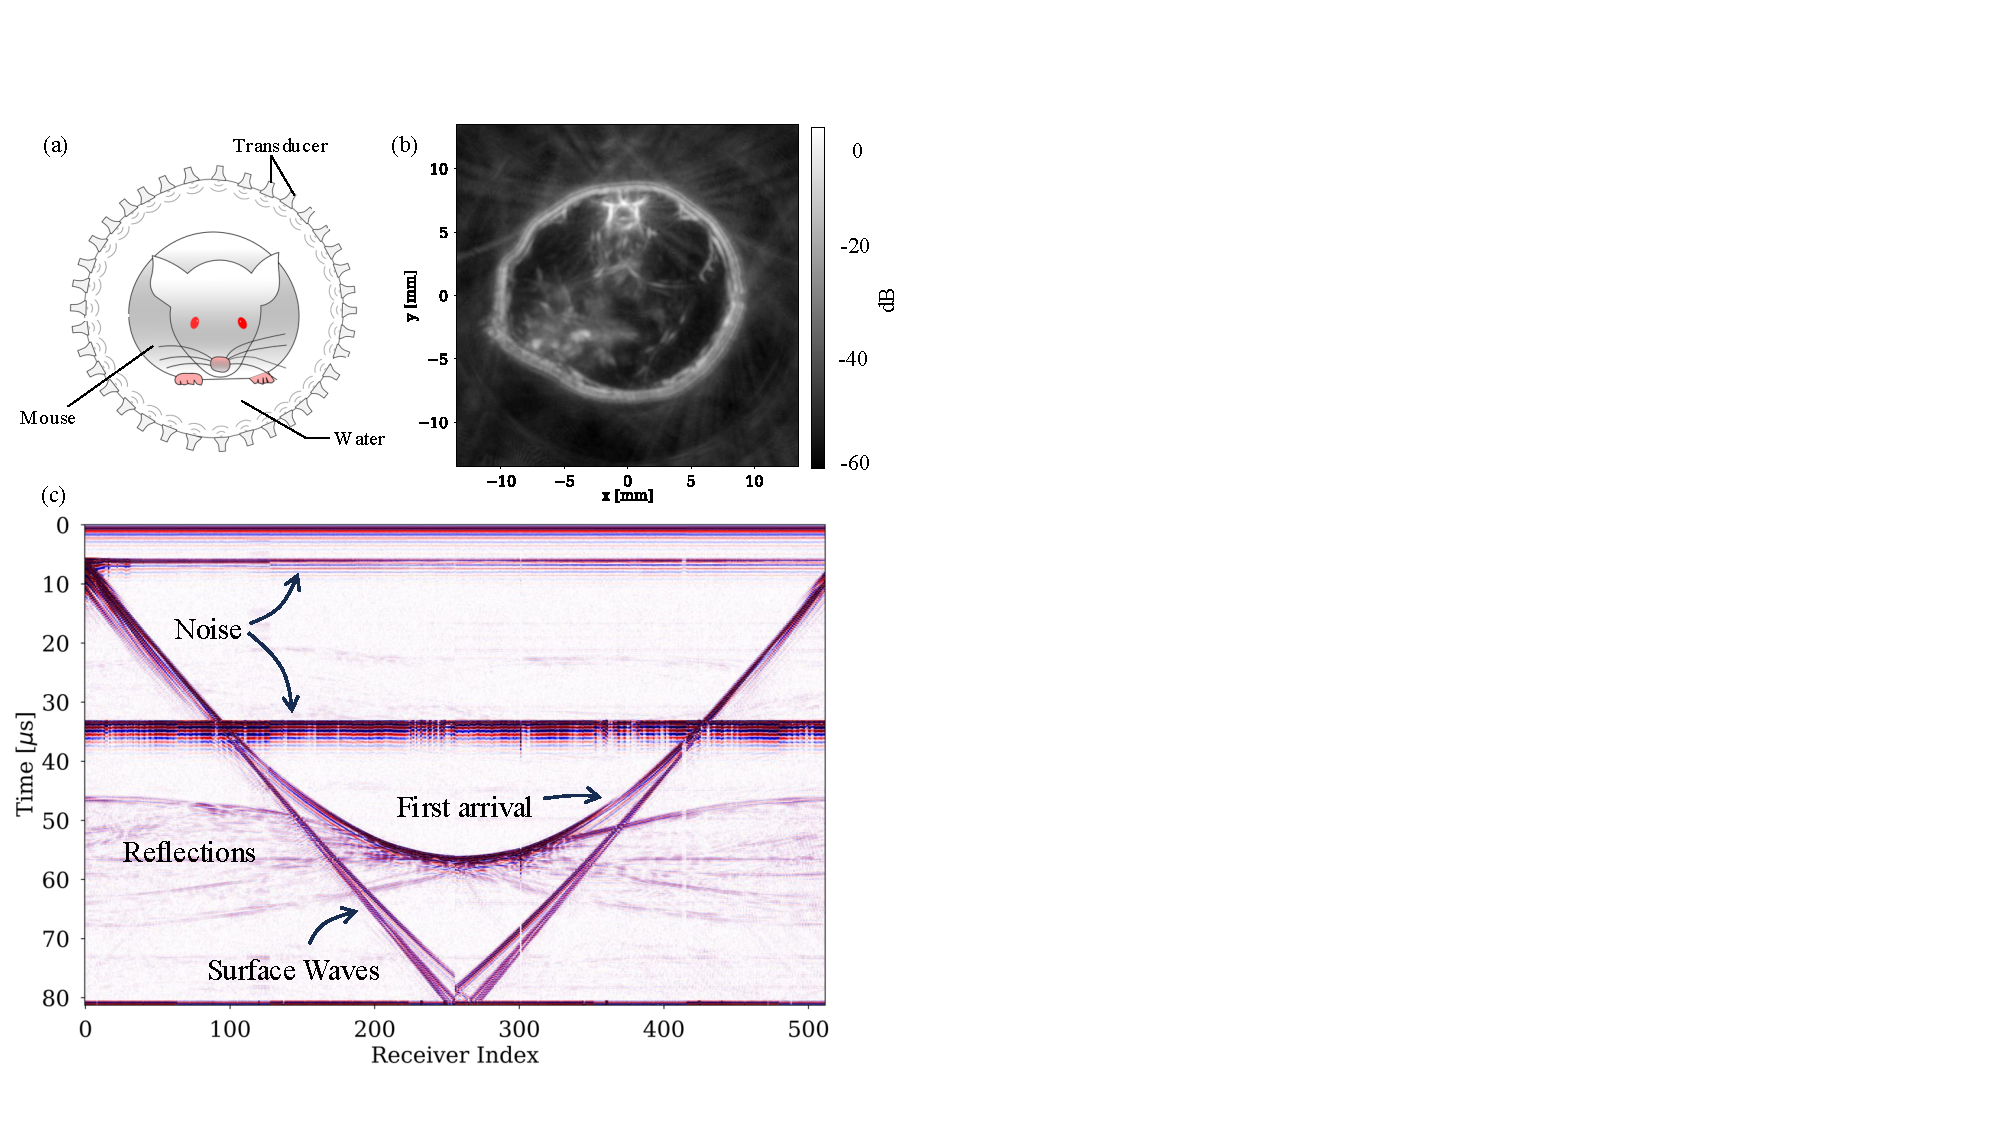
\includegraphics[width=0.8\textwidth]{figure2.pdf}
  \caption{(a) A schematic sketch (not to scale) of the imaging system. The mouse is anesthetized and immersed into a water bath during data acquisition. (b) Reflectivity image of the cross-sectional slice acquired with the delay-and-sum method. (c) Entire view of the bandpassed filtered data (750 kHz - 2.5 MHz) for one source, with traces stacked along the x-axis.}
  \label{fig:setup_shotgather_traces}
\end{figure}
%----------
%-----------------------------------------------------------------------------------
% Pre-processing
%-----------------------------------------------------------------------------------
\subsection{Pre-processing and data selection}
\Fref{fig:setup_shotgather_traces}(c) shows a full view of the bandpassed filtered data (750 kHz - 2.5 MHz) with an annotation of important events that will determine the data selection entering the inversion. First, between 0 to 7 $\mu$s, 30 to 40 $\mu$s and after 80 $\mu$s noise bands pollute the data. These bands arise from the impedance adjustment in the data acquisition system, which becomes necessary when switching from emission to reception mode. Furthermore, we note linear events that coincide with the first arrival for approximately the first and last fifth of the receivers. We expect these events to be related to surface waves propagating in the transducer ring that houses the individual transducer elements. To avoid mapping these effects into the reconstructed model a top mute is applied for all receivers up to 40 $\mu$s, and although this reduces the length of the signals used during the inversion drastically, all the information constraining the model parameters is contained in the events recorded after 40 $\mu$s. Additionally, we apply a sliding window to remove the effect of the linear events that are visible after 40 $\mu$s for receivers 100 - 400 in \fref{fig:setup_shotgather_traces}(c).  
%-----------------------------------------------------------------------------------
% Inversion setup and results
%-----------------------------------------------------------------------------------
\subsection{Inversion setup and results}
\label{subsec:InversionandResults}
%---------- 
\begin{figure}[!h]
  \centering
  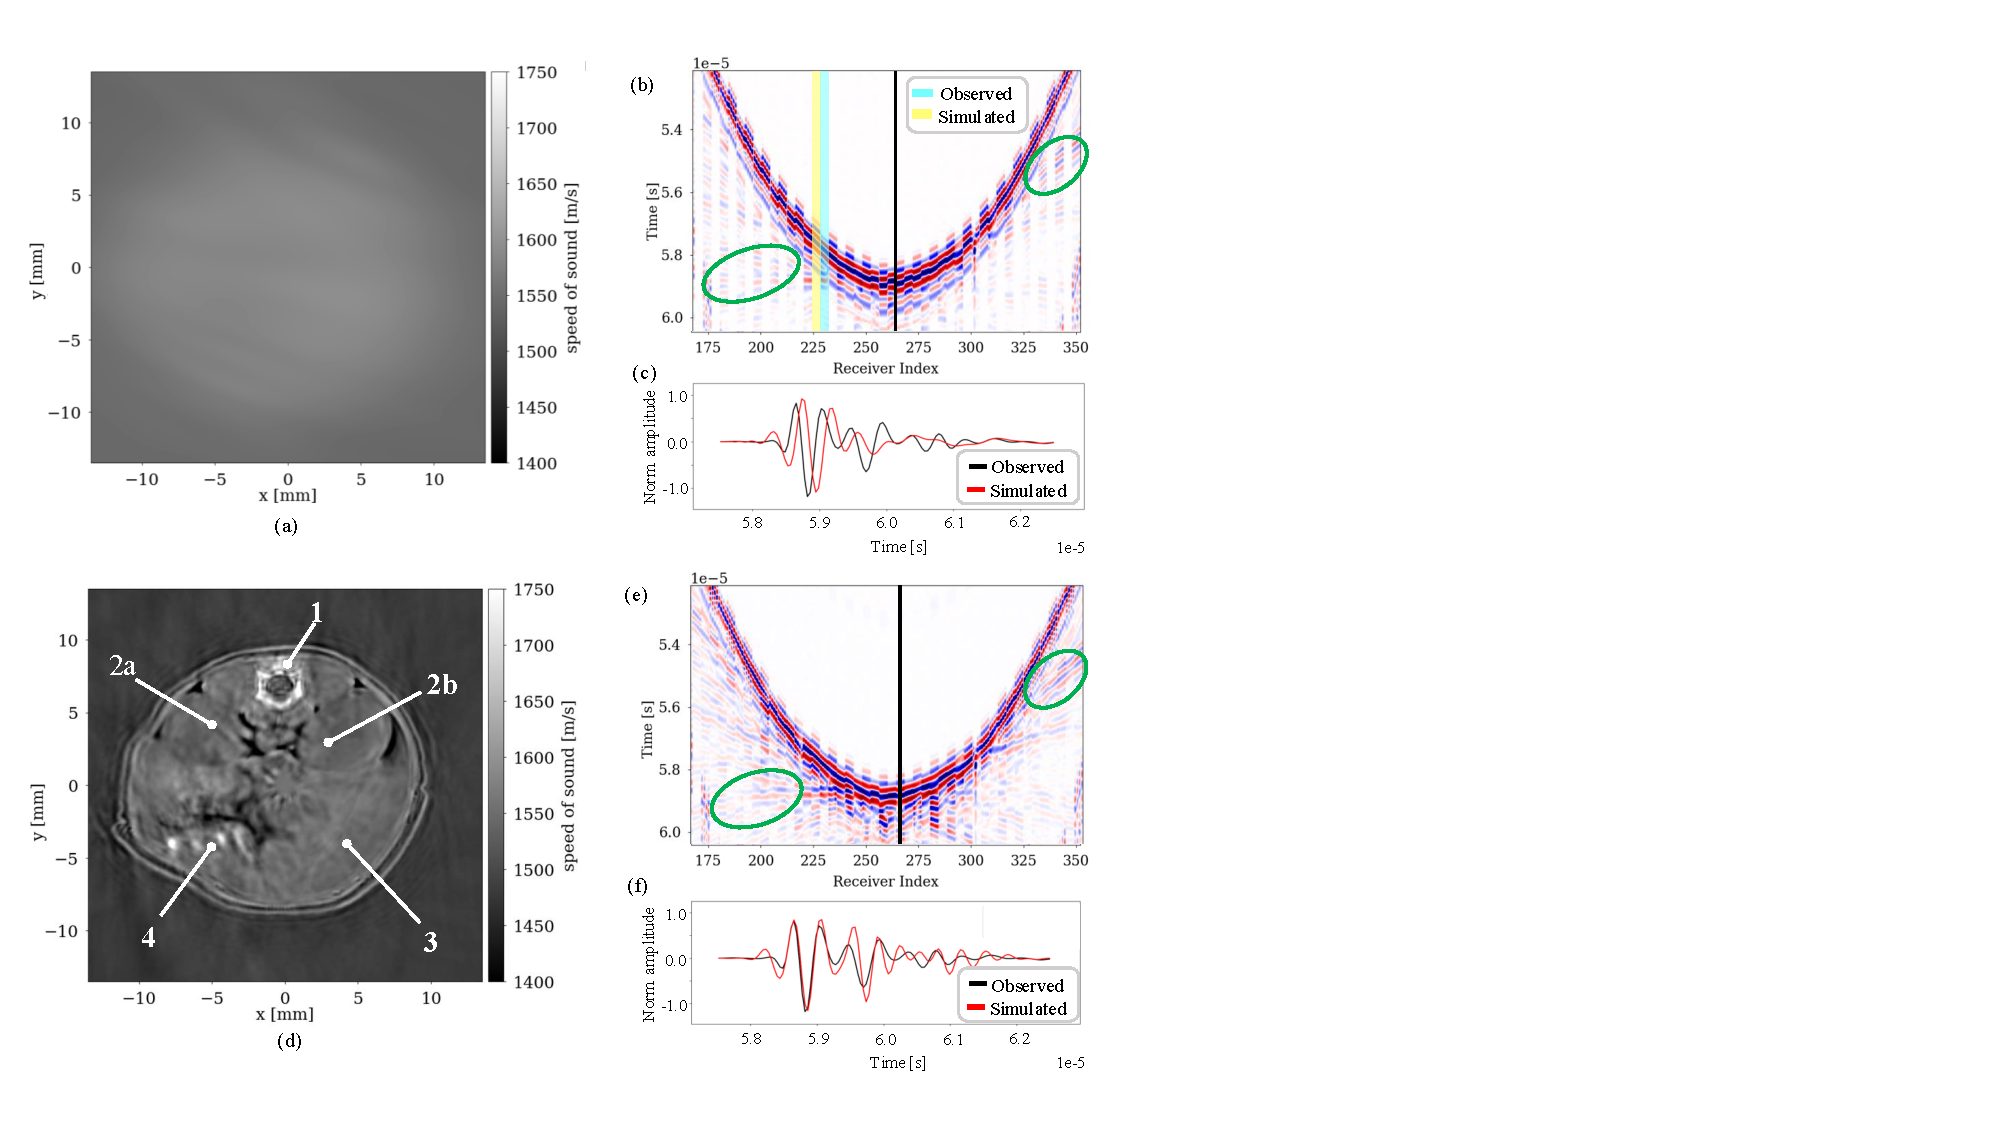
\includegraphics[width=\textwidth]{figure3.pdf}
  \caption{(a) Initial model derived from a straight-ray reconstruction. (b) Interwoven A-scan gather of transmission data showing 10 traces from the measured data at the frequency band 750 kHz - 2.5 MHz and 10 traces from the initial model alternatingly. (c) Waveform fit for the receiver marked by the black line in (b). (d) Final model for the frequency band 750 kHz - 2.5 MHz. Reconstructed features are (1) the vertebral column, (2a) right kidney, (2b) left kidney, (3) spleen and (4) liver. (e) Same as for (b), but comparing the measured data at the final frequency band 750 kHz - 2.5 MHz and the data from the final model displayed in (d). (f) same as for (c) but for the final fit. Green circles in (b) and (e) mark areas where the filled in reflections are well visible.}
  \label{fig:recons_and_repaired_shotgather}
\end{figure}
%----------
Once the data are windowed, we start the FWI workflow, which consists of: (1) an initial model derived from a straight-ray inversion, (2) an auxiliary inversion to recover individual source-time functions, (3) a multiscale scheme, where the frequency content is successively increased in three steps starting with a frequency band at 750 kHz to 1.5 MHz and ending with 750 kHz to 2.5 MHz, and (4) the implementation of the graph-space optimal transport to define the misfit measure. To reduce the computational load inherent to time domain approaches for applications with a large number of sources, batches of 64 sources are used per iteration and exchanged throughout the inversion such that full coverage of the domain is ensured. Since the aperture is circular, we choose the batches systematically to consist of every 8th transducer and shift this selection by one transducer per iteration. To calculate one model update and hence one iteration at the last frequency band (including frequencies up to 2.5 MHz) using 64 sources and the aforementioned data selection takes about 30 minutes on an HPC cluster using 72 GPUs (Nvidia Tesla P100). Across all frequency bands, a total of 330 iterations were performed. 

\Fref{fig:recons_and_repaired_shotgather}(a) displays the starting model and (d) shows the final inverted sound speed model with labeled reconstructed features such as the vertebral column (1), the kidneys (2), the spleen (3) and the liver (4). The quality of the reconstruction becomes also apparent upon comparison of \fref{fig:recons_and_repaired_shotgather}(b) with \fref{fig:recons_and_repaired_shotgather}(e). These figures show interleaved A-scan gathers, where four traces of the measured data filtered at the last frequency band 750 kHz to 2.5 MHz are plotted in alternance with four traces of simulated data though the initial model in (a) or the model at the final iteration in (d). Not only have the wavefronts been adjusted correctly in most cases, but also the reflections are completed properly, which is highlighted by the green circles. Both of these features are also visualized in the waveform fit in \fref{fig:recons_and_repaired_shotgather}(c) and (f) respectively, which displays the trace marked by the black line in the A-scan gathers.
%---------- 
\begin{figure}[!h]
  \centering
  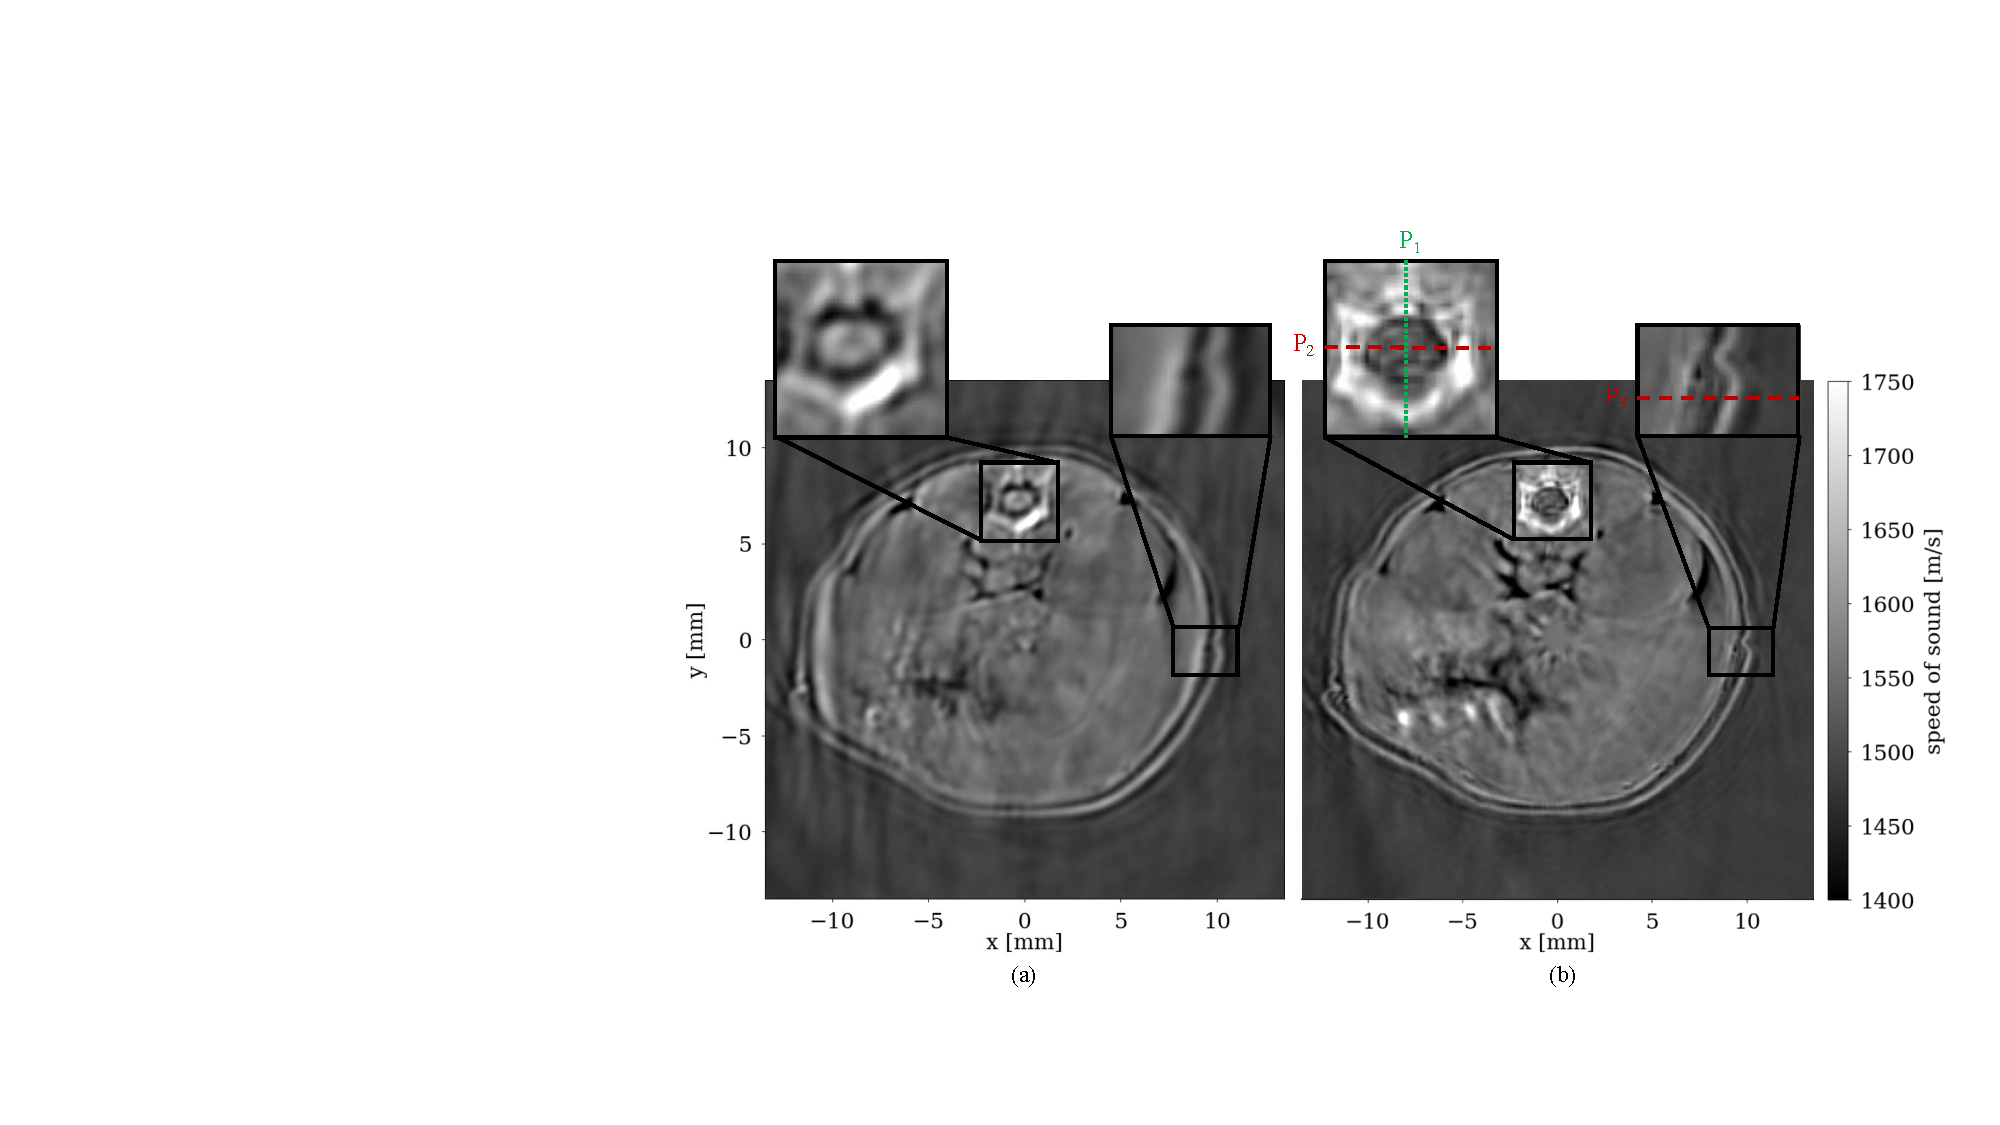
\includegraphics[width=\textwidth]{figure4.pdf}
  \caption{(a) The inverted sound speed model with an approximated source-time function and (b) the inverted model obtained when using the calibrated source-time function from section \ref{subsec: source_inversion}. Profiles P$_1$, P$_2$ and P$_3$ are shown in \fref{fig:ProfilePlots}.}
  \label{fig:Compare_estimatesSTF_invertedSTF_withProfiles}
\end{figure}
%----------

We have previously stressed the importance of calibrating the source wavelet in order to improve the waveform fit. This increase in accuracy directly translates into improved spatial resolution of the reconstructed models, as illustrated in \fref{fig:Compare_estimatesSTF_invertedSTF_withProfiles}. Comparing the model obtained by using an estimated source wavelet, averaged from the first arrival through water in \fref{fig:Compare_estimatesSTF_invertedSTF_withProfiles}(a), to the model that utilizes the calibrated source-time functions in \fref{fig:Compare_estimatesSTF_invertedSTF_withProfiles}(b), one notes an increase in image sharpness as well as a decrease of spatial artifacts, for instance the vertical line to the left in \fref{fig:Compare_estimatesSTF_invertedSTF_withProfiles}(a).

%-----------------------------------------------------------------------------------
% Multistage inversion
%-----------------------------------------------------------------------------------
\subsection{Multistage inversion for reflection and transmission tomography}
Images that capture accurate structural information are in practice as valuable as quantitative images, which motivates the implementation of a multistage inversion that reconstructs not only sound speed images, but also reflection images with RTM. Building on the same physics driven approach as FWI, RTM solves the wave equation \eref{eq:wave_equation_time_domain} via numerical wavefield simulations. If a homogeneous background medium is employed, Korta Martiartu \textit{et al.} \cite{Korta_Martiartu_2019} have shown that the forward operators in RTM and delay-and-sum are equivalent, assuming the same spatial and temporal discretizations have been used. \Fref{fig:Comparisonfig_RTM}(a) shows the impedance kernel, obtained with RTM for a homogeneous background model, which may be compared to \fref{fig:setup_shotgather_traces}(b) showing the reflectivity image obtained with standard delay-and-sum. 

The benefit of a more accurate physical wave propagation model only reveals itself when feeding a heterogeneous, more accurate sound speed distribution as the background model to the RTM task chain. This warrants that the backpropagated wavefield only interferes constructively with the forward wavefield at those locations that mark actual impedance contrasts within the medium. High-frequency variations in the sound speed model can lead to misalignment in interference patterns, resulting in inaccurate imaging of reflectors \cite{Davydenko_Verschuur_2021}. To ensure that constructive interference only occurs at actual scatterer locations, two preprocessing steps are often applied in practice: (1) muting the direct wave, which does not contain any reflection information and (2) ensuring that the background model is accurate, but not too detailed. The latter suggests either the use of a low-frequency reconstruction, or a smoothed version of the reconstructed model as a prior for RTM. Although it might be surprising that a smooth prior would lead to sharper reflection image, it is a logical consequence of RTM being based on backpropagation. A detailed model will generate many events that need to be mapped by the backpropagation operator. Obtaining such an exact operator is difficult if not impossible and any additional events that cannot be mapped correctly will appear as artifacts such as multiples. A smooth model without sharp boundaries, however, does not generate a large number of reflection events besides the first reflection arrival. Therefore, the corresponding backpropagation operator for a smooth model will primarily contain the initial arrival belonging to the first reflected wave, which is what we mostly rely on in reflection imaging.

Following this argumentation, we applied a diffusion-based smoothing operator with a smoothing length of half a wavelength (0.6 mm at 2.5 MHz) to the final model in \fref{fig:recons_and_repaired_shotgather}(d). Feeding this smoothed reconstruction as a background model to the RTM task chain results in \fref{fig:Comparisonfig_RTM}(b). The vertebrae, being a highly reflective bone structure, benefits the most from the more accurate sound speed background in terms of spatial resolution. The reflectors in the area of the kidneys are also more clearly depicted. Notably, the two strong point reflectors in the area of the liver, seen in \fref{fig:Comparisonfig_RTM}(a) as well as the sound speed reconstruction \fref{fig:recons_and_repaired_shotgather}(b), are almost invisible and substituted by a more complex structure. 
 %---------- 
\begin{figure}[!h]
    \centering
    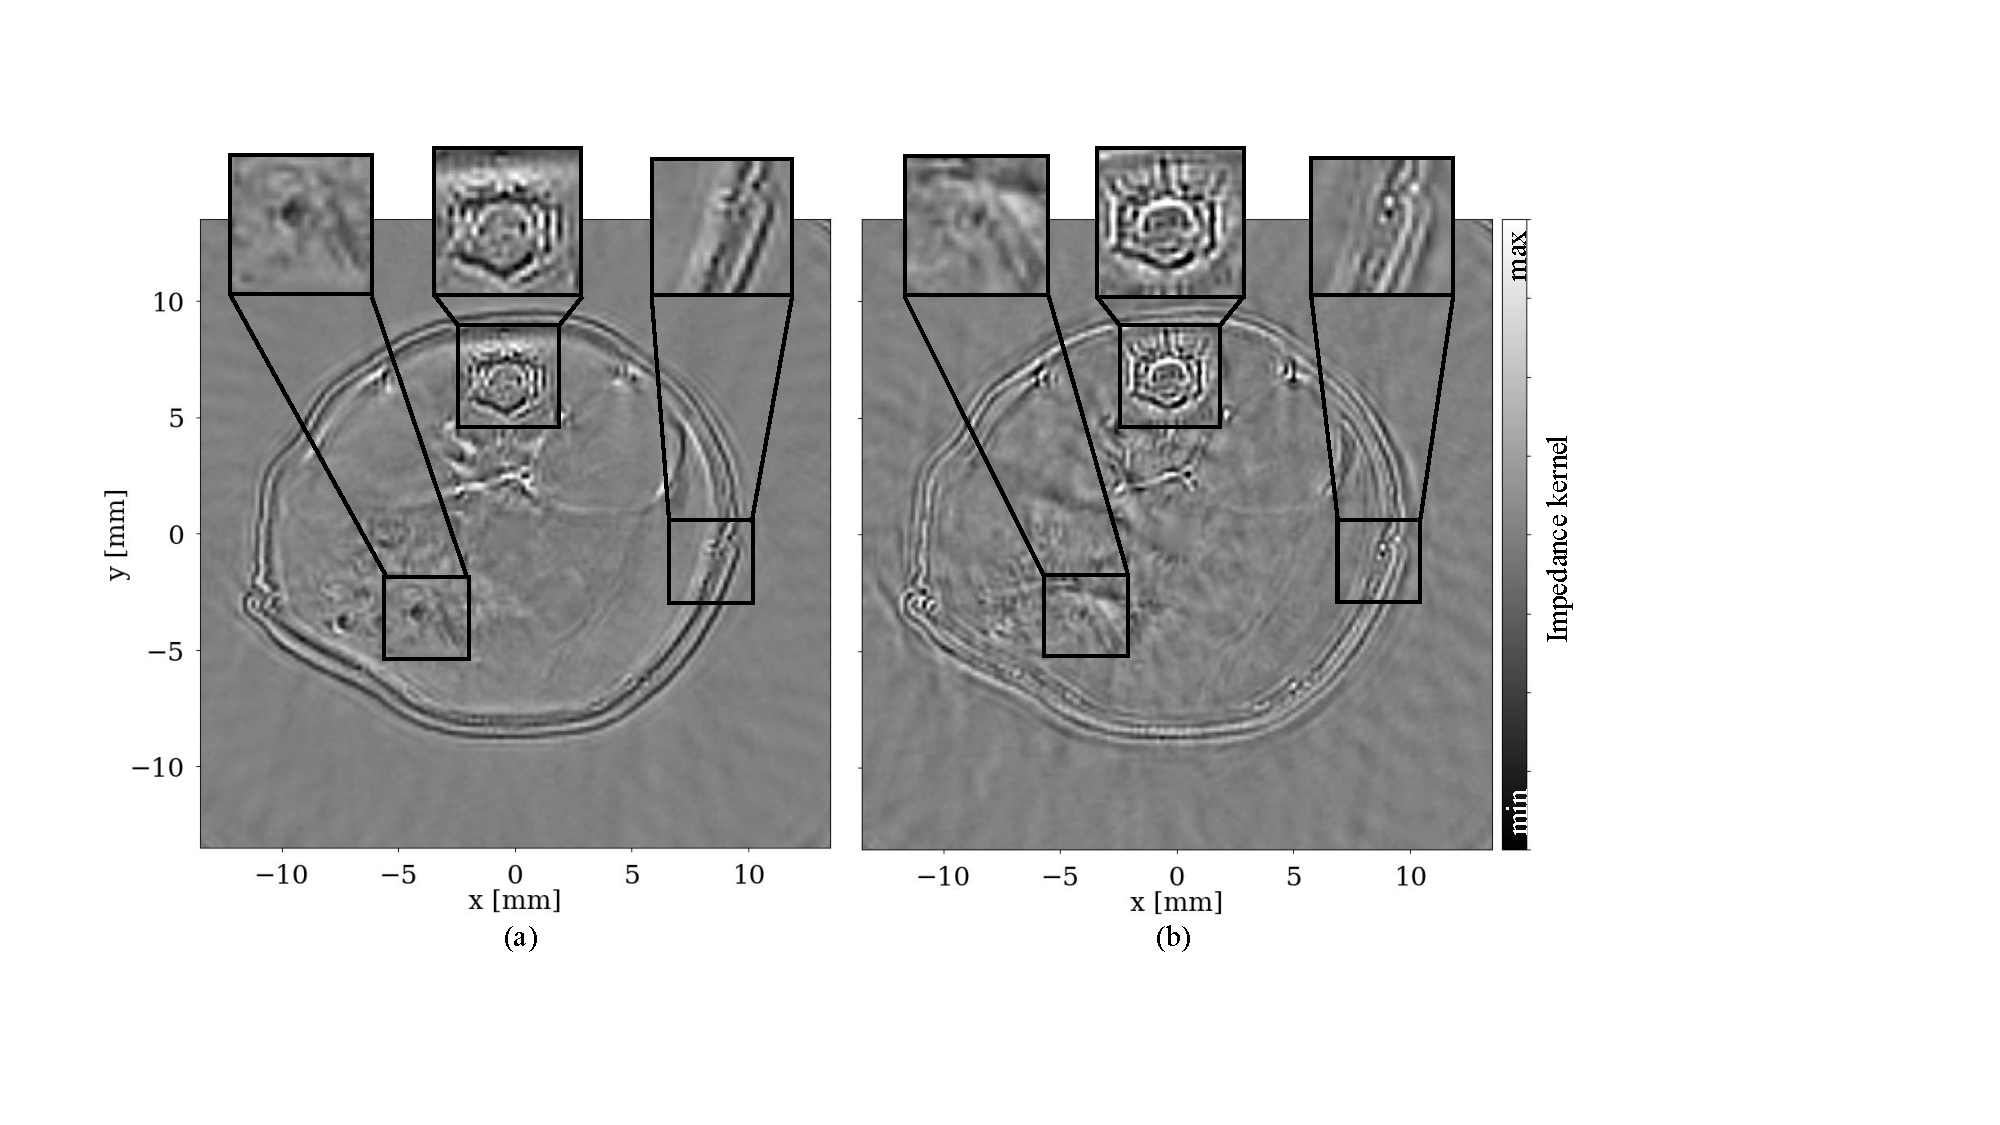
\includegraphics[width=\textwidth]{figure5.pdf}
    \caption{(a) The impedance kernel, a reflection image, obtained with RTM using a homogeneous background model; (b) The impedance kernel obtained with the reconstructed sound speed distribution shown in \fref{fig:recons_and_repaired_shotgather}(b) as the background model.}
    \label{fig:Comparisonfig_RTM}
\end{figure}
%----------

%-----------------------------------------------------------------------------------
% Resolution analysis
%-----------------------------------------------------------------------------------
\subsection{Resolution analysis}
\label{subsec:resolution_analysis_results}
To assess the spatial accuracy of the sound speed reconstruction, we propose a twofold approach: first, we will analyze reconstructed features directly in pixel space. Second, we will investigate the resolution in model space by characterizing the spatial blurring of point perturbations. We start with the profile plots P$_1$ and P$_2$ across the vertebrae in fref{fig:ProfilePlots}, which demonstrate that the osseous vertebral column with sound speed values around 1940 m/s is clearly separated from the lower sound speed values of the surrounding soft tissue around 1540 m/s as well as from the vertebral canal with sound speed values around 1520 m/s. To measure the spatial accuracy of an isolated feature, we focus on a zoomed-in region of the skin layer and determine the full width at half maximum (FWHM) value of profile P$_3$ to be 0.28 mm, which falls within the range of values reported for epidermal thickness in mice \cite{Caetano_2016}. 
 %---------- 
 \begin{figure}[!h]
    \centering
    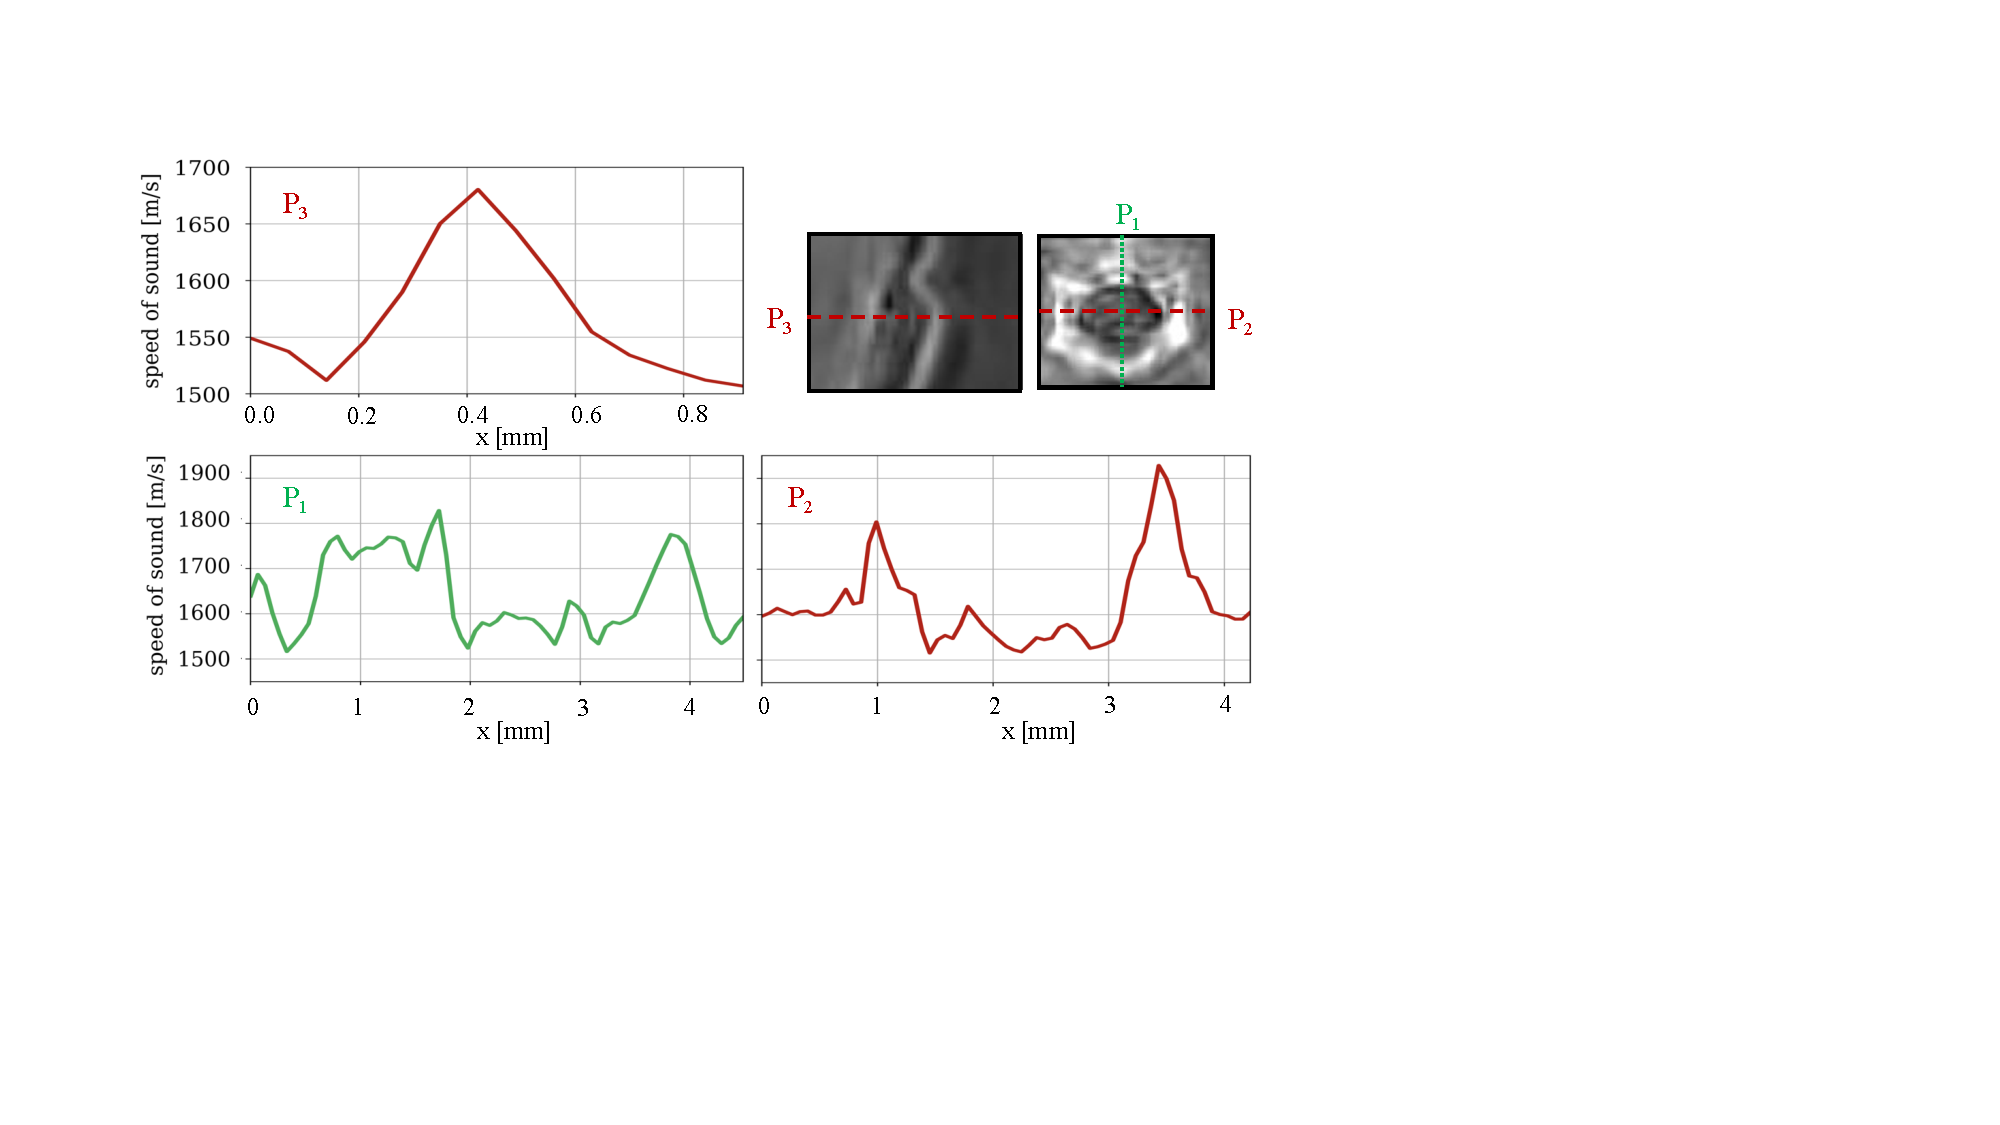
\includegraphics[width=\linewidth]{figure6.pdf}
    \caption{Profile plots across the zoomed-in region on the vertebral column and profile plot across the skin layer from \fref{fig:Compare_estimatesSTF_invertedSTF_withProfiles}.}
    \label{fig:ProfilePlots}
\end{figure}
%----------

The second approach to estimate resolution lengths is model based and follows the recipe presented in section \ref{subsec:resolution_analysis}. We start by inserting a set of low-velocity point perturbations with a strength of 30 \% from the surrounding sound speed values in the reconstructed model at various locations as shown in \fref{fig:mouseperturbation_PSFs}(a). These point perturbations have a diameter of 0.25 mm, which is on the order of half a wavelength for a background velocity of 1540 m/s at 2.5 MHz. Using this perturbed model, Hessian-vector products for five encoded sources instead of the entire 512 original sources are calculated and summed, which results in the image shown in \fref{fig:mouseperturbation_PSFs}(b). Following \eref{eq:Hesse-vector_product}, the Hessian-vector product indicates the direction of a single-iteration model update and is considered as a conservative estimate of the point-spread-function (PSF) \cite{Fichtner_Leeuwen_2015}. Given that the reconstructed model lies in the vicinity of the optimal model, \eref{eq:Hesse-vector_product} can be approximated by one gradient computation. In the context of our source encoding procedure, this implies that one needs to compute as many gradients as encoded sources per perturbed model. These gradients are then summed to reduce the cross-talk noise introduced by the encoded sources. Since we use five encoded sources, we sum five encoded gradients to obtain the image in \fref{fig:mouseperturbation_PSFs}(b).
 %---------- 
 \begin{figure}[!h]
    \centering
    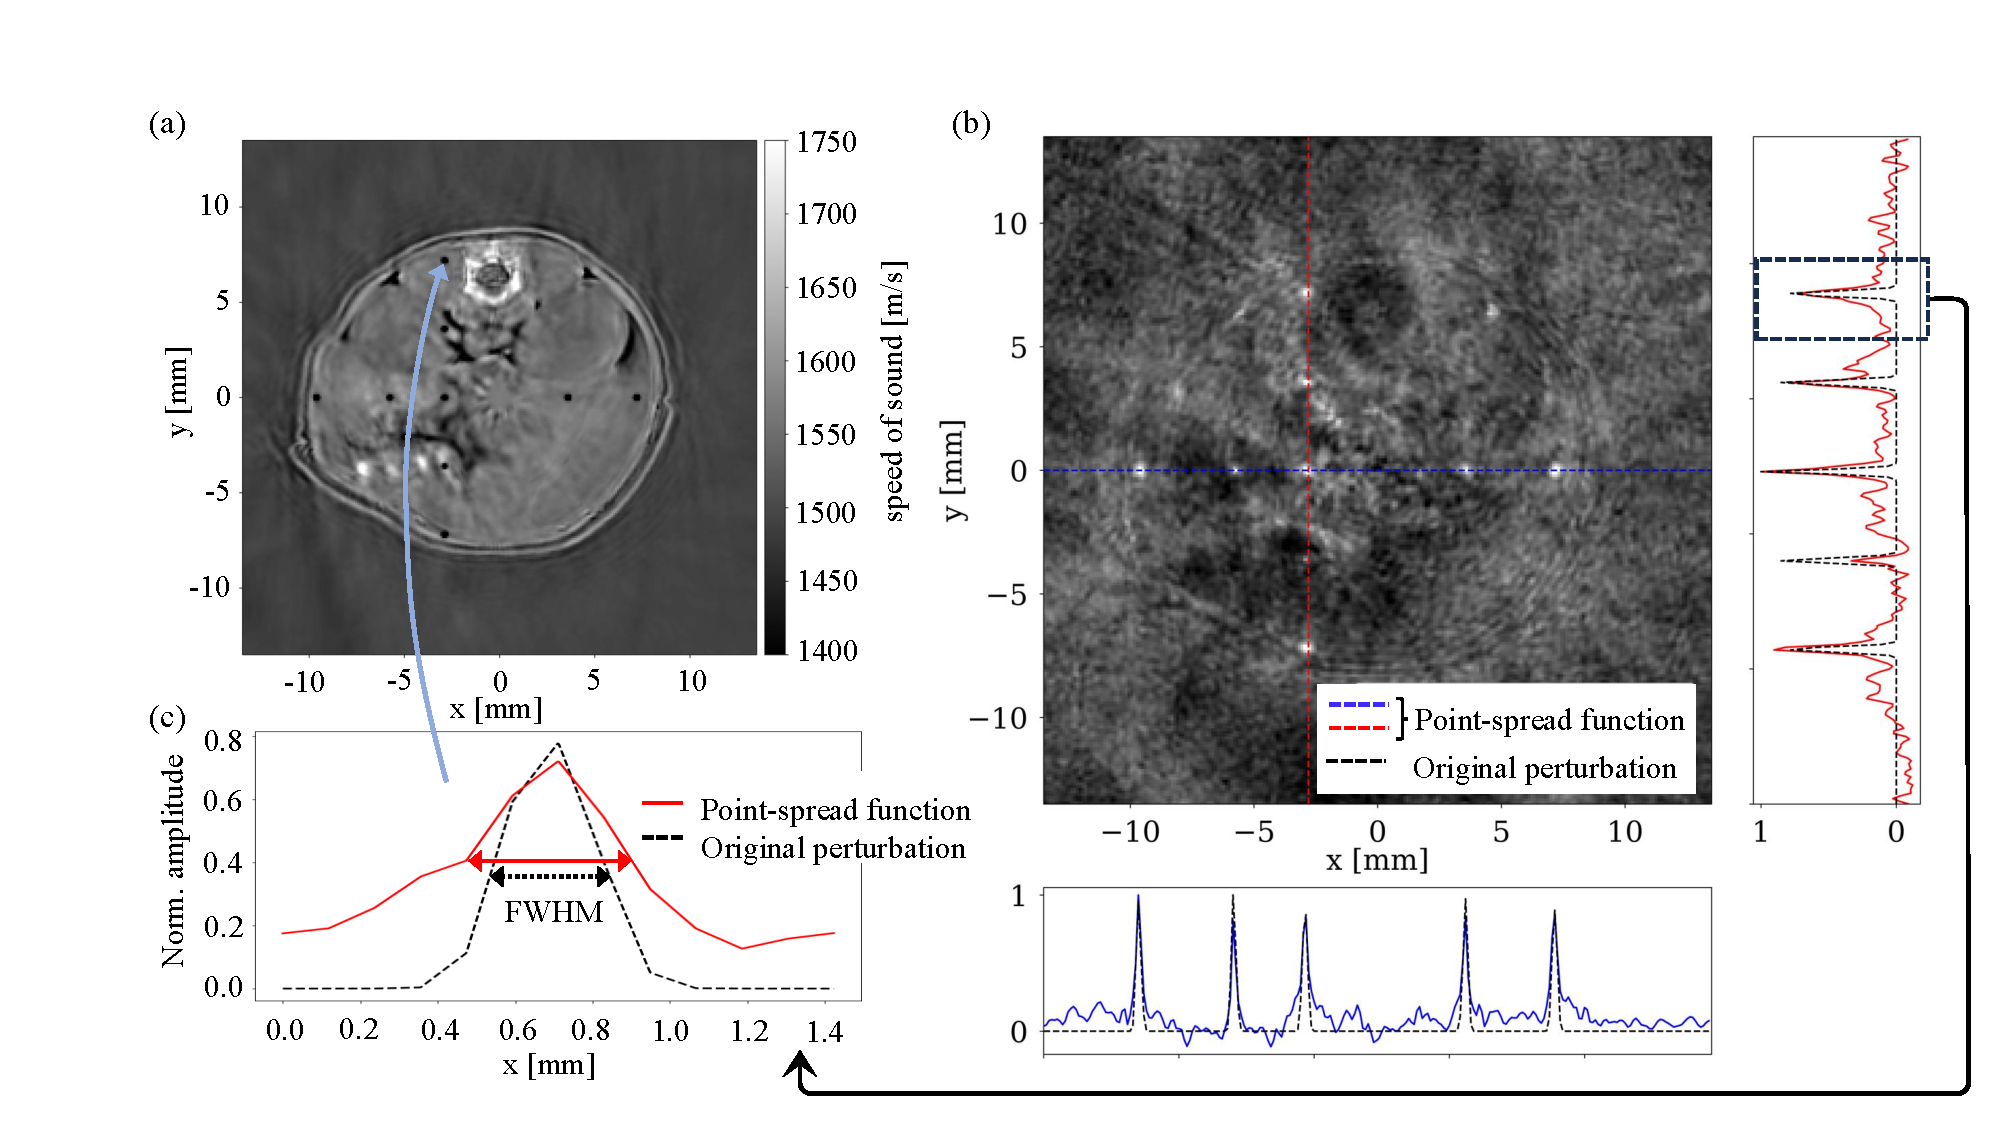
\includegraphics[width=\textwidth]{figure7.pdf}
    \caption{(a) Point perturbations with a diameter of half a wavelength and a strength of 30 \% from the surrounding values inserted in the FWI reconstructed model; (b) The gradient of the misfit with respect to the model parameters calculated from 5 encoded sources. The perturbations from (a) are clearly discernible. The profile plots show that the magnitude of the imaged perturbation is space dependent, which indicates that not all areas are resolved equally well; (c) A zoom on a PSF with the FWHM measure indicated.}
    \label{fig:mouseperturbation_PSFs}
\end{figure}
%---------- 
The imprint of the model in the gradient in \fref{fig:mouseperturbation_PSFs}(b) is clearly discernible, and the inserted low velocity perturbations appear expectedly as bright spots, indicating that the sound speed at these points needs to be increased in order to fit the measurements. Taking the profiles along the vertical (red line) and horizontal (blue line) perturbations and comparing them to their original size (black line) provides a proxy for the spread of the individual peak, which may, for instance, be calculated using the full width at half (FWHM) as indicated in \fref{fig:mouseperturbation_PSFs}(c). In this case, the FWHM of the original perturbation is equal to 0.29 mm, while the FWHM of the PSF is 0.56 mm. Averaging the FWHM values for all five vertical perturbations suggests that the size of the perturbation has increased by approximately 30 \% in the PSFs compared to the original perturbation. Linking this to the theoretical, idealized noise-free resolution limit of FWI of half a wavelength, we find that for our real and thus noisy data, the spatial resolution is closer to one wavelength. Additionally, comparing amplitudes provides further information on the local resolution. We note that the spread as well as the amplitude of the point perturbations within the perturbed gradient varies for each location and is especially affected in the vicinity of scatterers, such as the top perturbation near the point inserted inside the high velocity structure in the liver.

Owing to the time shift introduced to construct the encoded sources, the encoded simulations are approximately 10 times longer than an individual simulation, however, since we only use 5 encoded sources the computation time for this resolution analysis with encoded sources is still reduced by a factor 10, compared to using the original sources.
    
To evaluate the effect of a large sound speed difference between the background and the perturbation, we test two scenarios in \fref{fig:Vertebrae_perturbation}, showing the perturbed model in the upper row and the corresponding gradient below. The most prominent scatterer of the model is the vertebral column, a bone structure with reconstructed sound speed values on the order of 1940 m/s. Here, waves are strongly scattered due to the large sound speed contrast and inserting a small perturbation with a diameter of around half a wavelength for a maximum frequency at 2.5 MHz as seen in \fref{fig:Vertebrae_perturbation}(a) will solely have a small effect on the scattering behavior and therefore does not appear in the corresponding gradient in \fref{fig:Vertebrae_perturbation}(b). In contrast, moving the perturbation inside the vertebral canal in \fref{fig:Vertebrae_perturbation}(c), where the sound speed difference with respect to the background medium is smaller, leads to a clear imprint of the perturbation in the gradient in \fref{fig:Vertebrae_perturbation}(d).  
 %---------- 
 \begin{figure}[!h]
    \centering
    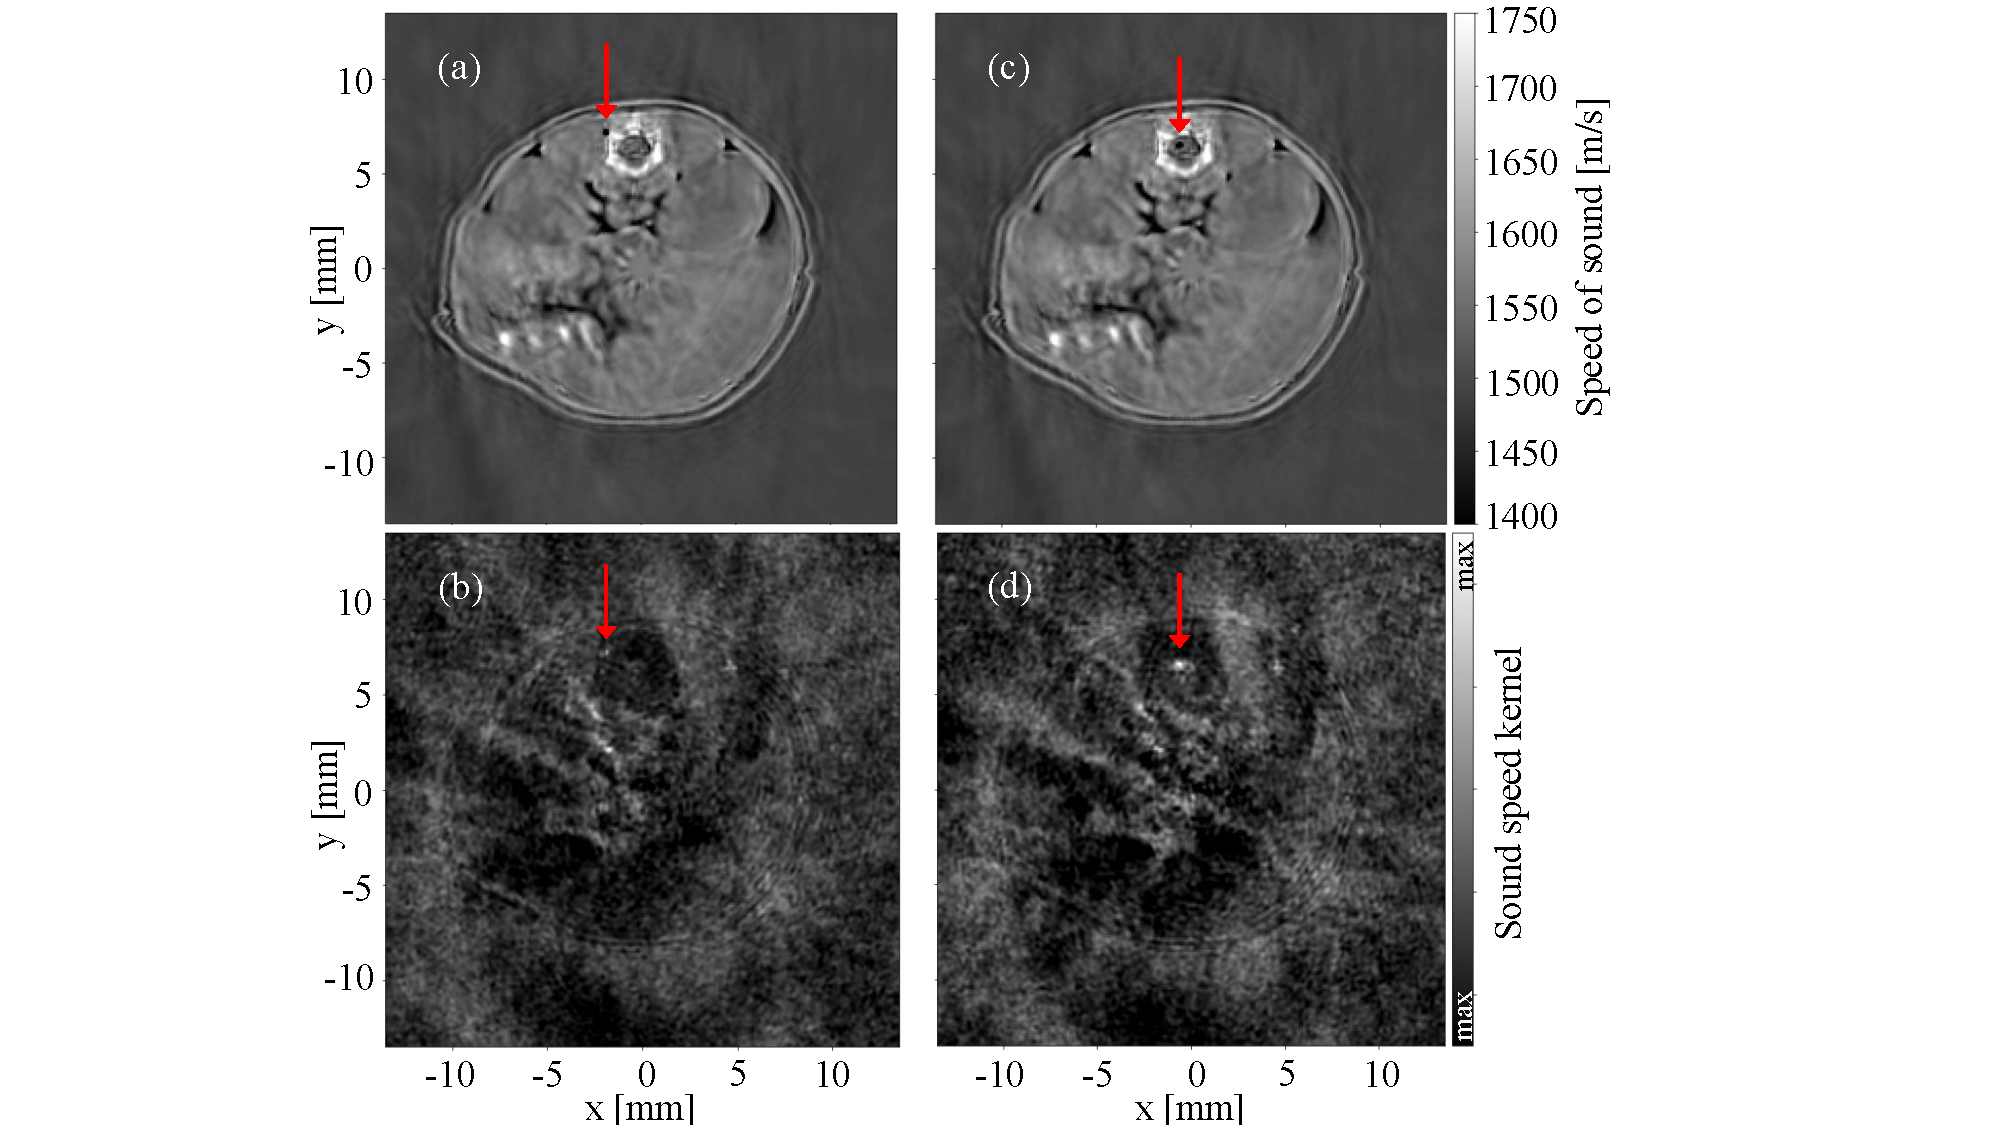
\includegraphics[width=0.8\textwidth]{figure8.pdf}
    \caption{Point perturbations of various size, inserted in regions of the model with a large sound speed difference between the perturbation and the background medium. (a) Low sound speed perturbation with a diameter of half a wavelength, inserted at the edge of the vertebrae, a high sound speed scatterer. (b) In the corresponding gradient, the perturbation is not discernible. (c) Low sound speed perturbation with a diameter of half a wavelength inside the vertebral canal. (d) Due to the reduced sound speed difference between the background and the perturbation, the latter is clearly visible in the gradient.}
    \label{fig:Vertebrae_perturbation}
\end{figure}
%----------    
Approximating resolution lengths via gradient perturbation using source stacking provides a conservative estimate of resolution lengths and may serve as a quick, minimum quality check and can be readily automated. This would equip the clinical practitioner with the possibility to swiftly assess the resolution of individual reconstructed features. The workflow may, however, be easily adapted to analyze the resolution quality of local features to greater extend by (1) iterating on the perturbed models to improve the sharpness of the point perturbations, (2) increasing the number of encoded wavefields, and (3) using more sophisticated source-encoding methods to minimize the cross-talk, for instance by using phase shifts \cite{Tromp_Bachmann_medicalEncoding_2020}. 

%-----------------------------------------------------------------------------------
% Quantitative tissue characterisation
%-----------------------------------------------------------------------------------
\subsection{Quantitative tissue characterization in the presence of high contrast}
Although the inversion scheme uses the acoustic wave equation and is thus strictly speaking only correct for soft tissues with negligible elasticity, the reconstructed shape and sound speed values of the vertebral column on the order of 1940 m/s are significantly higher than values for soft tissue, as expected for the sound speed in bones \cite{ITIS_database}. This provides a potential new perspective for ultrasound computed tomography (USCT): orthopedic imaging. Presently, to our best knowledge, there exists no USCT system in clinical practice for orthopedic imaging due to the difficulty to handle the high impedance contrast between bone and soft tissue. This difficulty primarily stems from the fact that in common ultrasound tomography, the forward problem in \eref{eq:wave_equation_time_domain} is linearized and is thus only valid when perturbations are large relative to the wavelength such that diffraction effects are negligible. In the presence of bone, this linear approximation is inadequate and will produce artifacts. Wiskin \textit{et al.} \cite{Wiskin_boneUS_2020} have shown the capability of transmission ultrasound tomography to produce high-resolution images in the presence of bone when using a wave-based imaging approach. In this case, the modelling accounts for both the nonlinearity of the problem and all wave phenomena. The reconstruction of the vertebral column in this study further highlights the potential of wave-based ultrasound tomography for orthopedic imaging with applications for instance in sports medicine or in the context of osteoporosis treatment.  

%=======================================================================================
%%%%%%%%%% CONCLUSION %%%%%%%%%%
%=======================================================================================
\section{Conclusions}
In this study, we apply FWI to in-vivo data, which remains to this date challenging due to the nonlinearity and computational complexity of the problem. We condense the success of the reconstruction procedure to the following key features: (1) a misfit functional based on graph-space optimal transport that provides a robust measure for waveform differences in time and amplitude, which alleviates the occurrence of local minima and helps to steer the inversion towards the global minimum; (2) an auxiliary inversion to calibrate the source-time functions provides an essential ingredient to accurately simulate the ultrasonic wavefield. Once an accurate sound speed distribution has been reconstructed, it can be employed as a background model in reflection imaging with RTM to enhance the sharpness of reflectors. This workflow thus provides both quantitative insights into model parameter values and qualitative, structural information. We have shown that, despite the acoustic approximation used in the FWI model, we are able to reconstruct sound speed values for both soft tissue and the osseous vertebral column, which fall within the expected range of values from the literature. These results are further augmented by a practical strategy for resolution analysis that complies with the requirements for dense source-receiver apertures commonly used in real applications. Point-spread functions thereby provide proxies to test the local resolution of the tomographic model and show that we are able to image structures smaller than one wavelength at the maximum frequency. These resolution tests are relatively cheap to compute and can be automated, which makes them especially appealing for practical applications. We expect the combination of the proposed methods to be in particular valuable to further promote the benefits of FWI for medical ultrasound. 




\section*{References}
\bibliographystyle{jphysicsB} % Choose your preferred bibliography style
\bibliography{report} % Name of your .bib file without the extension
\end{document}

